\documentclass{article}
\usepackage[utf8]{inputenc}
\usepackage[a4paper, total={6in, 8in}]{geometry}
\usepackage{xcolor,colortbl}

\title{Búsqueda local}
\author{Eric Dacal, Joaquim Marset, Josep de Cid}
\date{Marzo 2017}

\usepackage{natbib}
\usepackage{graphicx}

\definecolor{DarkGrey}{HTML}{DFDFDF}
\definecolor{LightGrey}{HTML}{F2F2F2}

\begin{document}

\maketitle

\section{Preguntas}
\begin{enumerate}
  \item \textbf{¿Qué elementos intervienen en el problema?}
  \begin{itemize}
      \item \textbf{Sensores:} Son nodos con la capacidad de tanto transmitir como recibir información. Tienen la capacidad de envio de datos limitada a 3 veces la cantidad de información que pueden captar, que puede oscilar entre 1MB/s, 2MB/s o 5MB/s. Tienen las conexiones entrantes limitadas a tres. Se distribuyen aleatoriamente por el mapa dependiendo de la semilla de generación.
      \item \textbf{Centros:} Son nodos con la capacidad de recibir hasta veinticinco conexiones entrantes y no permiten enviar información ya que son el destino final de esta. Al igual que con los sensores, su distribución también es aleatoria.
  \end{itemize}
  \item \textbf{¿Cuál es el espacio de búsqueda?}\par
  Todas las posibles soluciones que cumplan las restricción de mantener todos los sensores conectados.
  \item \textbf{¿Qué tamaño tiene el espacio de búsqueda?}\par
  ----
  \item \textbf{¿Qué es un estado inicial?}\par
  La primera solución válida a partir de la cual se va ejecutar el algoritmo de IA.
  \item \textbf{¿Qué condiciones cumple un estado final?}\par
  ----
  \item \textbf{¿Qué operadores permiten modificar los estados?}
  \begin{itemize}
      \item \textbf{\textit{Swap}:} ----
      \item \textbf{\textit{Switch}:} ----
  \end{itemize}
  \item \textbf{¿Qué factor de ramificación tienen los operadores de cambio de estado?}
  \begin{itemize}
      \item \textbf{\textit{Swap}:} ----
      \item \textbf{\textit{Switch}:} ----
  \end{itemize}
\end{enumerate}

\section{Experimentos}
\begin{enumerate}
  % PREGUNTA 1
  \item \textbf{Determinar qué conjunto de operadores da mejores resultados para una función heurística que optimice el criterio de calidad del problema (3.2) con un escenario en el que el número de centros de datos es 4 y el de sensores es 100. Deberéis usar el algoritmo de Hill Climbing. Escoged una de las estrategias de inicialización de entre las que proponéis. A partir de estos resultados deberéis fijar los operadores para el resto de experimentos. Pensad que con estas proporciones, se podrán transmitir todos los datos.}

  % PREGUNTA 2
  \item \textbf{Determinar qué estrategia de generación de la solución inicial da mejores resultados para la función heurística usada en el apartado anterior, con el escenario del apartado anterior y usando el algoritmo de Hill Climbing. A partir de estos resultados deberéis fijar también la estrategia de generación de la solución inicial para el resto de experimentos.}

  Un elemento importante en un problema de búsqueda local es la influencia del estado de partida en el coste de la solución final ya que puede decrementar drásticamente el número de pasos al acercarse a la solución óptima. Se han diseñado las siguientes estrategias de generación de soluciones iniciales:
  \begin{itemize}
    \item \textbf{Dummy Sequential:} Genera una solución inicial donde cada sensor se conecta con el siguiente sin ordenarlos de ninguna forma, tal y como se genera la lista con la semilla dada, hasta que el último sensor se conecta al centro de datos.
    \item \textbf{Simple Greedy:} Genera una solución inicial ordenando todos los sensores por su capacidad en orden decreciente y siguiendo el orden, conectar cada uno con el primer nodo de mayor capacidad que permita más conexiones (priorizando centros de datos ya que tienen capacidad ilimitada).
    \item \textbf{Distance Greedy:} Al igual que el \textit{Simple Greedy}, genera una solucion ordenando los sensores por capacidad decreciente, y como diferencia, en este se conecta al nodo de mayor capacidad que se encuentre más cerca del sensor.
  \end{itemize}

  A priori no se puede llegar a determinar si un estado inicial es mejor o peor ya que se desconoce el espacio de búsqueda. Para probar la hipótesis debemos realizar un experimento donde se debe garantizar que cada prueba se realiza en las mismas condiciones. Para ello se han realizado diez réplicas del experimento, donde se prueba cada estado inicial descrito, y para ello se va a realizar cada experimento individual con la misma semilla de números aleatorios para así garantizar que cada prueba tenga una configuración de sensores y centros idéntica en cada uno de los diferentes estados iniciales.\par

  En este caso, la solución de cada experimento no es comparable, ya que cada réplica parte de condiciones distintas, así que se deben tomar otros datos como la calidad de la solución o el tiempo que se tarda en obtenerla, normalmente magnitudes correlacionadas. Con todo esto, el experimento puede ser resumido en los siguientes puntos:
  \begin{itemize}
    \item \textbf{Observación:} Pueden haber estados iniciales que obtienen mejores soluciones que otros.
    \item \textbf{Planteamiento:} Se escogen diversos métodos de generación de estados iniciales y se observan sus soluciones.
    \item \textbf{Hipótesis:} Todos los métodos de inicialización son iguales (H\textsubscript{0}), o hay estados mejores que otros (H\textsubscript{1}).
    \item \textbf{Método experimentación:} \begin{itemize}
        \item Elegir 10 semillas de generación aleatorias, una para cada réplica.
        \item Ejecutar un experimento para cada semilla para la inicialización, con 100 sensores y 4 centros de datos para \textit{Dummy Sequential}, \textit{Simple Greedy} y \textit{Distance Greedy}.
        \item Usar el algoritmo de \textit{Hill Climbing} y medir coste, información, tiempo y nodos expandidos para realizar la comparación.
    \end{itemize}
  \end{itemize}

  Se pueden observar los datos generados en cada réplica en la siguiente tabla, dónde las estratégias de generación aparecen representadas por sus siglas DS (\textit{Dummy Sequential}), SG (\textit{Simple Greedy}) y DG (\textit{Distance Greedy}):
  \begin{center}
    \begin{tabular}{ | r | r | r | r | r | r | r | r | r | r | }
      \hline
      \rowcolor{DarkGrey}
      & \multicolumn{3}{|c|}{Coste} & \multicolumn{3}{c|}{Expansiones} & \multicolumn{3}{|c|}{Tiempo} \\ \hline
      \rowcolor{DarkGrey}
      \multicolumn{1}{|c|}{Réplica} & \multicolumn{1}{|c|}{DS} & \multicolumn{1}{|c|}{SG} & \multicolumn{1}{|c|}{DG} & \multicolumn{1}{|c|}{DS} & \multicolumn{1}{|c|}{SG} & \multicolumn{1}{|c|}{DG} & \multicolumn{1}{|c|}{DS} & \multicolumn{1}{|c|}{SG} & \multicolumn{1}{|c|}{DG} \\ \hline \hline
      1 & 131871.0 & 125657.0 & 121535.0 & 145 & 129 & 88 & 8542 & 5842 & 4021 \\ \hline
      \rowcolor{LightGrey}
      2 & 192921.0 & 192636.0 & 184075.0 & 148 & 115 & 83 & 7039 & 5278 & 3728 \\ \hline
      3 & 146387.0 & 148113.0 & 144927.0 & 146 & 115 & 79 & 6888 & 5264 & 3529 \\ \hline
      \rowcolor{LightGrey}
      4 & 142036.0 & 138780.0 & 139212.0 & 154 & 129 & 81 & 7207 & 5805 & 3728 \\ \hline
      5 & 224573.0 & 210339.0 & 217941.0 & 145 & 123 & 75 & 6732 & 5563 & 3400 \\ \hline
      \rowcolor{LightGrey}
      6 & 334282.0 & 329574.0 & 315465.0 & 129 & 119 & 99 & 6190 & 5691 & 4526 \\ \hline
      7 & 210457.0 & 221211.0 & 200202.0 & 139 & 109 & 81 & 6680 & 4952 & 3743 \\ \hline
      \rowcolor{LightGrey}
      8 & 163742.0 & 169532.0 & 161120.0 & 130 & 141 & 81 & 6043 & 6809 & 3701 \\ \hline
      9 & 133242.0 & 139395.0 & 136800.0 & 149 & 113 & 83 & 7101 & 5165 & 3665 \\ \hline
      \rowcolor{LightGrey}
      10 & 182535.0 & 176715.0 & 177079.0 & 138 & 136 & 85 & 6622 & 6372 & 3937 \\ \hline
    \end{tabular}
  \end{center}

  \begin{figure}[htp]
    \centering
    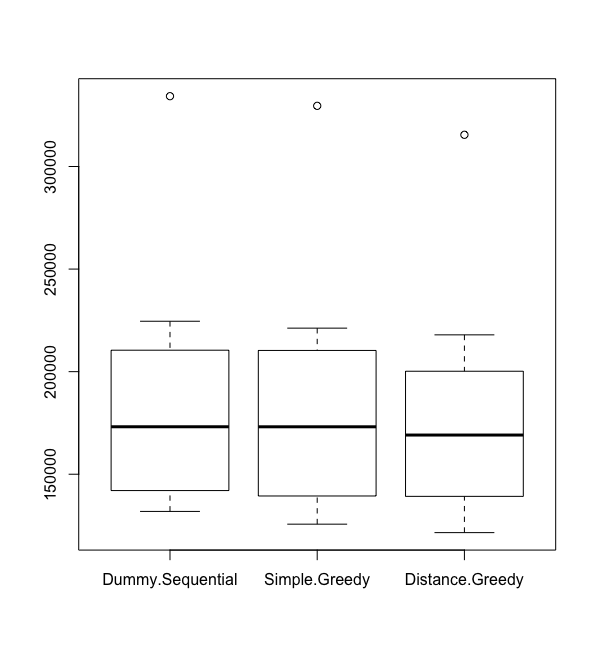
\includegraphics[width=.3\textwidth]{images/initialState_Cost_BP}\hfill
    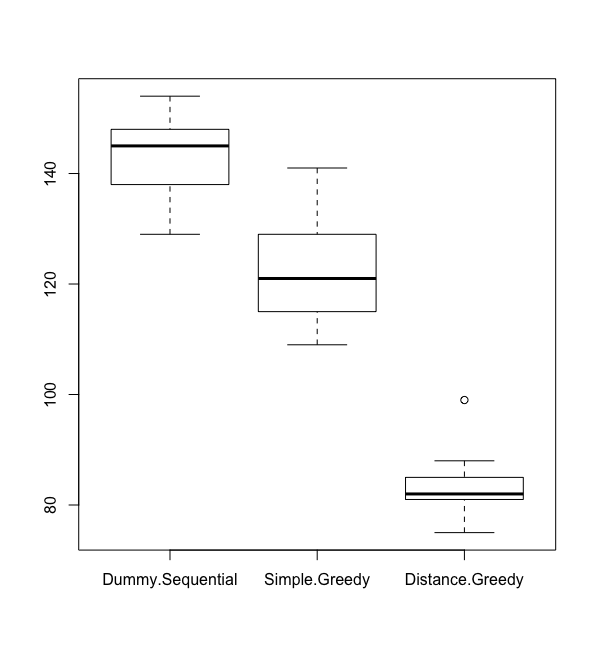
\includegraphics[width=.3\textwidth]{images/initialState_Expansions_BP}\hfill
    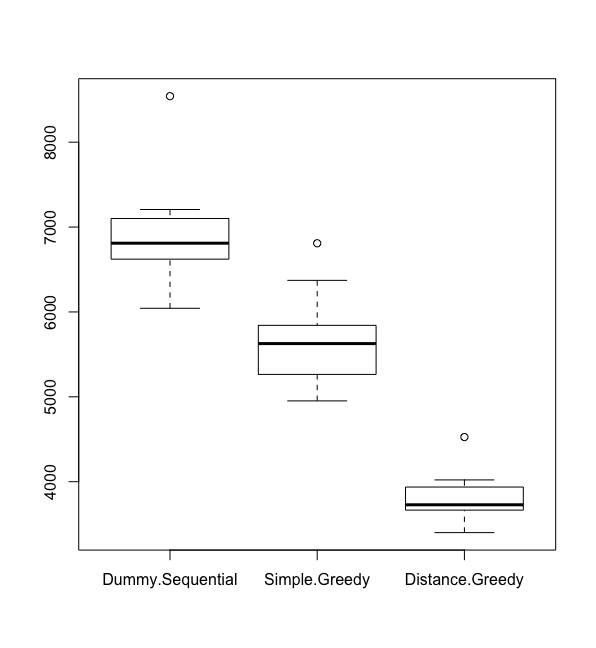
\includegraphics[width=.3\textwidth]{images/initialState_Time_BP}
    \caption{\textit{Boxplots con los datos de coste, expansiones y tiempo respectivamente}}
  \end{figure}

  A partir de los datos, se han generado los \textit{Boxplots} de la Fig.1, que será desde donde van a ser analizados los datos y generadas las conclusiones, tratando los datos sin tener en cuenta algunos \textit{outliers} que aparecen con una probabilidad remota debido a la aleatoriedad de los experimentos.\par
  En cuanto a coste final no se observa gran diferencia (ya que está más ligado a los operadores) aunque el \textit{Distance Greedy} consigue una pequeña mejora del coste, con una media de 179835.6, respecto a los 186204.6 del \textit{Dummy Sequential} y los 185195.2 del \textit{Simple Greedy}. Por ello, dejando de lado el coste final que se obtiene, se comparan los resultados por cada pareja de estados iniciales, considerando la probabilidad de que un método de generación de mejores soluciones que los otros para un experimento que se distribuye en forma de función binomial y así comprobar cual es la probabilidad de que la hipótesis nula sea cierta.

  \begin{itemize}
    \item \textbf{Dummy Sequential - Simple Greedy:} En esta pareja se ve claramente que el \textit{Simple Greedy} da mejores resultados tanto en tiempo como en número de expansiones, por lo que consultamos en la tabla binomial la probabilidad de que en 10 experimentos, el \textit{Simple Greedy} gane en 9 de ellos, suponiendo que las dos estrategias son iguales. Con la resta de las intersecciones [n=10, x=9, p=0.5] y [n=10, x=8, p=0.5] se obtiene que la probabilidad es de 0.0097, por lo que no es cierto que los dos métodos sean iguales, cosa que implica que \textit{Simple Greedy} sea considerado mejor.
    \item \textbf{Dummy Sequential - Distance Greedy:} En este caso se repite el entorno de antes con aún más diferenciada la mejora que presenta el \textit{Distance Greedy}, dando una probabilidad aún más pequeña, de 0.001, así que damos por demostrado que este se considera mejor.
    \item \textbf{Simple Greedy - Distance Greedy:} En este último caso se vuelve a repetir el entorno anterior, con la misma probabilidad de 0.001, por lo que también se considera como mejor el \textit{Distance Greedy}.
  \end{itemize}

  Cómo conclusión, se puede afirmar que la estrategia de generación \textit{Distance Greedy} es la que genera mejor estado inicial, y es la que se va a usar a partir de ahora en los siguientes experimentos. Aunque en coste está a la par con los otros dos métodos, es claramente mejor en cuestión de tiempo y expansiones, por lo que se puede suponer que la solución inicial generada deja la configuración mucho más cerca de un mínimo.

  \item \textbf{Determinar los parámetros que dan mejor resultado para el Simulated Annealing con el mismo escenario, usando la misma función heurística y los operadores y la estrategia de generación de la solución inicial escogidos en los experimentos anteriores.}

 \begin{itemize}
    \item \textbf{Observación:} Pueden haber variables que obtengas mejores resultados para Simulated Annealing.
    \item \textbf{Planteamiento:} Escogemos una variable,fijamos el resto escogiendo valores aleatorios para ellas y vamos variando sequenciamente el valor escogido.
    \item \textbf{Hipótesis:} Todas los valores para los parametros de inicialización son iguales (H\textsubscript{0}), o hay valores mejores que otros (H\textsubscript{1}).
    \item \textbf{Método experimentación:} \begin{itemize}
        \item Elegir 10 semillas de generación aleatorias, una para cada réplica.
        \item Ejecutar13 experimento para cada semilla para la inicialización, ¿? \textit{Dummy Sequential}, \textit{Simple Greedy} y \textit{Distance Greedy}.
        \item Usar el algoritmo de \textit{Hill Climbing} y medir coste, información, tiempo y nodos expandidos para realizar la comparación.
    \end{itemize}
  \end{itemize}


  \item \textbf{Dado el escenario de los apartados anteriores, estudiad como evoluciona el tiempo de ejecución para hallar la solución para valores crecientes de los parámetros siguendo la proporción 4:100. Comenzad con 4 centros de datos e incrementad el número de 2 en 2 hasta que se vea la tendencia. Usad el algoritmo de Hill Climbing y la misma función heurística que antes.}

  \item \textbf{Las proporciones del primer escenario hacen que la capacidad de recibir datos sea mucho mayor que la de captura. A partir de todos los experimentos realizados, ¿hay resultados en los que no todos los centros de datos son utilizados? Si es el caso, estimad la proporción centros de datos/sensores que indican los experimentos.}

  \item \textbf{Suponiendo que los centros de datos no sean costosos, podríamos estimar como afecta el añadir más centros al coste de la red. Fijando el numero de sensores en 100, realizad experimentos aumentando el número de centros de datos de dos en dos hasta 10 y medid el coste de la red de conexión, el número de centros de datos usados y el coste temporal para hallar la solución. Usad el algoritmo de Hill y el de Simulated Annealing. Climbing.}

  \item \textbf{En el escenario que habéis explorado esta prácticamente asegurado el transmitir todos los datos, eso hace que el factor de la función heurística que maximiza los datos transmitidos no tenga casi efecto durante la búsqueda (es constante la mayor parte del tiempo) y que solo se tenga en cuenta el coste de la red de distribución. Ahora cambiaremos el escenario de manera que haya dos centros de datos y 100 sensores. Para buscar soluciones en este escenario, ajustad la función heurística de manera que se puedan dar distintos pesos al factor que mide la cantidad de información enviada. Usad el algoritmo de Hill Climbing en estos experimentos y responded a las siguientes preguntas:}
  \begin{itemize}
    \item \textbf{¿Se ha reducido el tiempo para hallar una solución?}
    \item \textbf{Si usamos una ponderación para el factor que mide la cantidad de información enviada igual que en los primeros escenarios ¿En que proporción aumenta el coste de la red?}
    \item \textbf{¿Cómo cambia el coste de la red en función de la ponderación que se da al envío de los datos?}
    \item \textbf{¿Hay una ponderación a partir de la que el coste de la red ya no aumenta?}
  \end{itemize}
\end{enumerate}
\end{document}